\section[Path-Independent Vector Fields]{Path-Independent Vector Fields and the Fundamental Theorem of
Calculus for Line Integrals} \label{S:12.4.FTCLI}


\vspace*{-14 pt}
\framebox{\hspace*{3 pt}
\parbox{6.25 in}{\begin{goals}
\item How can we characterize the vector fields $\vF$ for which
  $\int_C\vF\cdot d\vr$ has the same value for every oriented path
  from a point $P$ to a point $Q$?
\item What special properties do gradient vector fields have?
\end{goals}} \hspace*{3 pt}}

\subsection*{Introduction}

In some of the activities and examples in this chapter we have
encountered situations where $C_1$ and $C_2$ are different oriented curves from a
point $P$ to a point $Q$ and $\int_{C_1}\vF\cdot d\vr =
\int_{C_2}\vF\cdot d\vr$. In this section, we explore vector fields
which have the property that for all points $P$ and $Q$, if $C_1$ and
$C_2$ are oriented paths from $P$ to $Q$, then $\int_{C_1}\vF\cdot
d\vr = \int_{C_2}\vF\cdot d\vr$.

\begin{pa} \label{PA:12.4}

In Activity~\ref{A:12.3.2} we considered the vector field $\vF(x,y) =
\langle y^2,2xy+3\rangle$ and two different oriented curves from
$(1,0)$ to $(-1,0)$. We found that the value of the line integral of
$\vF$ was the same along those two oriented curves.
\ba
\item Verify that $\vF(x,y) = \langle y^2,2xy+3\rangle$ is a gradient
  vector field by showing that $\vF = \nabla f$ for the function
  $f(x,y) = xy^2 + 3y$.
\item Calculate $f(-1,0)-f(1,0)$. How does this value compare to the
  value of the line integral $\int_{C_1}\vF\cdot d\vr$ you found in
  Activity~\ref{A:12.3.2}?
\item Let $C_3$ be the line segment from $(1,1)$ to $(3,4)$. Calculate
  $\int_{C_3}\vF\cdot d\vr$ as well as $f(3,4)-f(1,1)$. What do you
  notice?
\saveCount
\ea

We've used Clairaut's Theorem to argue that a vector field in $\R^2$
is not a gradient vector field when $\partial F_1/\partial
y\neq \partial F_2/\partial x$, and earlier in this preview activity,
you verified that a given vector field was the gradient of a
particular function of two variables. Clairaut's Theorem holds for
functions of three variables. However, in that case there are six mixed partials to
calculate, and thus it can be rather tedious. The remaining parts of
this preview activity suggest a process for determining if a vector
field in $\R^3$ is conservative as well as finding a potential
function for the vector field.

Let $\vG(x,y,z) = \langle 3e^{y^2}+z\sin(x),6xy e^{y^2} -
  z,3z^2-y-\cos(x)\rangle$ and $\vH(x,y,z) = \langle 3x^2 y,x^3+2yz^3,xz+3y^2z^2\rangle$.
\ba
\restoreCount
\item If $\vG$ and $\vH$ are to be gradient vector fields, then there
  are functions $g$ and $h$ for which $\vG = \nabla g$ and $\vH=\nabla
  h$. What would this tell us about the partial derivatives $g_x$,
  $g_y$, $g_z$, $h_x$, $h_y$, and $h_z$?
\item Find a function $g$ so that $\partial g/\partial x =
  3e^{y^2}+z\sin(x)$. Find a function $h$ so that $\partial
  h/\partial x = 3x^2y$.
\item When finding the most general antiderivative for a function of
  one variable, we add a constant of integration (usually denoted by
  $C$) to capture the fact that any constant will vanish through
  differentiation. When taking the partial derivative with respect to
  $x$ of a function of
  $x$, $y$, and $z$, what variables can appear in terms that vanish
  because they are treated as constants? What does this tell you
  should be added to $g$ and $h$ in the previous part to make them
  the most general possible functions with the desired partial
  derivatives with respect to $x$?
\item Now calculate $\partial g/\partial y$ and $\partial
  h/\partial y$. Explain why this tells you that we must have
  \[g(x,y,z) = 3xe^{y^2}-z\cos(x)-yz+m_1(z)\]
  and
  \[h(x,y,z) = x^3y+y^2z^3+m_2(z)\]
  for some functions $m_1$ and $m_2$ depending only on $z$.
\item Calculate $\partial g/\partial z$ and $\partial h/\partial z$
  for the functions in the part above. Notice that $m_1$ and $m_2$ are
  functions of $z$ alone, so taking a partial derivative with respect
  to $z$ is the same as taking an ordinary derivative, and thus you
  may use the notation $m'_1(z)$ and $m'_2(z)$.
\item Explain why $\vG$ is a gradient vector field but $\vH$ is not a
  gradient vector field. Find a potential function for $\vG$.
\ea
\end{pa} 
\afterpa 
%%% Local Variables:
%%% mode: latex
%%% TeX-master: "../0_AC_MV"
%%% End:


\subsection*{Path-Independent Vector Fields}

We say that a vector field $\vF$ defined on a domain $D$ is
\textbf{path-independent} \index{pathindependent!definition} if
$\int_{C_1}\vF\cdot d\vr = \int_{C_2}\vF\cdot d\vr$ whenever $C_1$ and
$C_2$ are oriented paths in $D$ having the same initial point and same
terminal point. 

We've already encountered some situations where we had evidence that a
vector field was path-independent, but since the definition requires
that for every pair of points in the domain and every possible pair of
paths from oine point to the other we must get the same value, it
doesn't appear that verifying a vector field is path-independent is an
easy task. Fortunately, one familiar class of vector fields can be
shown to be path-independent. Let $f\colon \R^3\to \R$ be a function
for which $\nabla f$ is continuous on a domain $D$. Suppose that $P$
and $Q$ are points in $D$ and let $C$ be a smooth oriented path from $P$ to
$Q$. Let's take a look at $\int_C\nabla f \cdot d\vr$ by fixing an arbitrary
parameterization $\vr(t)$ of $C$, $a\leq t \leq b$. Since $\nabla
f(\vr(t)) = \langle f_x(\vr(t)),f_y(\vr(t)),f_z(\vr(t))\rangle$, we know that
\[\int_C\nabla f\cdot d\vr  = \int_a^b \nabla f(\vr(t))\cdot
\vr'(t)\, dt = \int_a^b \langle f_x(\vr(t)), f_y(\vr(t)),
f_z(\vr(t))\rangle \cdot \vr'(t)\, dt.\]
If $\vr(t) = \langle x(t), y(t), z(t)\rangle$, then the integrand
above is
\begin{multline*}\langle f_x(\vr(t)), f_y(\vr(t)), f_z(\vr(t))\rangle\cdot \langle
x'(t),y'(t),z'(t)\rangle =\\ f_x(x(t),y(t),z(t))x'(t) +
f_y(x(t),y(t),z(t))y'(t) + f_z(x(t),y(t),z(t))z'(t).\end{multline*}
Notice that this is exactly what the chain rule tells us
$\ds\frac{d}{dt} f(\vr(t))$ is equal to. Therefore,
\[\int_C\nabla f\cdot d\vr = \int_a^b \frac{d}{dt} f(\vr(t))\, dt =
f(\vr(b)) - f(\vr(a)) = f(Q) - f(P).\]
In other words, gradient vector fields are path-independent vector
fields, and we can evaluate line integrals of gradient vector fields
by using a potential function. (Technically the argument above assumed
that $C$ was smooth, but we can replace $C$ by a piecewise smooth
curve by splitting the line integral up into the sum of finitely many
line integrals along smooth curves.)

This result is so important that it is frequently called the
Fundamental Theorem of Calculus for Line integrals, because of its
similarity to the Fundamental Theorem of Calculus, which can be
written as
\[\int_a^b f'(x)\, dx = f(b) - f(a).\]
\vspace*{5pt}
\nin \framebox{\hspace*{3 pt}
  \parbox{6.25 in}{\textbf{Fundamental Theorem of Calculus for Line
      Integrals} Let $f$ be a function for which $\nabla f$ is
    continuous on a domain $D$. If $P$ and $Q$ are points in $D$ and
    $C$ is a piece-wise smooth oriented path from $P$ to $Q$ in $D$, then
  \[\int_C \nabla f\cdot d\vr = f(Q) - f(P).\]} \hspace*{3 pt}} \vspace*{5pt}

\begin{activity} \label{A:12.4.1}  
Calculate each of the following line integrals.
\ba
\item $\int_C \nabla f\cdot d\vr$ if $f(x,y) = 3xy^2 - \sin(x) + e^y$
  and $C$ is the top half of the unit circle oriented from $(-1,0)$ to $(1,0)$.
\item $\int_C \nabla g\cdot d\vr$ if $g(x,y,z) = xz^2 - 5y^3\cos(z) + 6$
  and $C$ is the portion of the helix $\vr(t) = \langle
  5\cos(t),5\sin(t),3t\rangle$ from $(5,0,0)$ to $(0,5,9\pi/2)$.
\item $\int_C \nabla h\cdot d\vr$ if $h(x,y,z) = 3y^2e^{y^3} -
  5x\sin(x^3z) + z^2$
  and $C$ is the curve consisting of the line segment from $(0,0,0)$
  to $(1,1,1)$, followed by the line segment from $(1,1,1)$ to
  $(-1,3,-2)$, followed by the line segment from $(-1,3,-2)$ to $(0,0,10)$.

\ea
\end{activity}
\begin{smallhint}

\end{smallhint}
\begin{bighint}

\end{bighint}
\begin{activitySolution}

\end{activitySolution}
\aftera
%%% Local Variables:
%%% mode: latex
%%% TeX-master: "../0_AC_MV"
%%% End:


By following the methodology laid out in Preview
Activity~\ref{PA:12.4} to show that a given vector field is a gradient
vector field, the Fundamental Theorem of Calculus for Line Integrals
makes evaluating a large number of line integrals simpler now.

\begin{activity} \label{A:12.4.1}  
Calculate each of the following line integrals.
\ba
\item $\int_C \nabla f\cdot d\vr$ if $f(x,y) = 3xy^2 - \sin(x) + e^y$
  and $C$ is the top half of the unit circle oriented from $(-1,0)$ to $(1,0)$.
\item $\int_C \nabla g\cdot d\vr$ if $g(x,y,z) = xz^2 - 5y^3\cos(z) + 6$
  and $C$ is the portion of the helix $\vr(t) = \langle
  5\cos(t),5\sin(t),3t\rangle$ from $(5,0,0)$ to $(0,5,9\pi/2)$.
\item $\int_C \nabla h\cdot d\vr$ if $h(x,y,z) = 3y^2e^{y^3} -
  5x\sin(x^3z) + z^2$
  and $C$ is the curve consisting of the line segment from $(0,0,0)$
  to $(1,1,1)$, followed by the line segment from $(1,1,1)$ to
  $(-1,3,-2)$, followed by the line segment from $(-1,3,-2)$ to $(0,0,10)$.

\ea
\end{activity}
\begin{smallhint}

\end{smallhint}
\begin{bighint}

\end{bighint}
\begin{activitySolution}

\end{activitySolution}
\aftera
%%% Local Variables:
%%% mode: latex
%%% TeX-master: "../0_AC_MV"
%%% End:


\begin{activity} \label{A:12.4.2}  
Calculate each of the following line integrals.
\ba
\item $\int_C \vF\cdot d\vr$ if $\vF(x,y) = \langle 2x,2y\rangle$
  and $C$ is the line segment from $(1,2)$ to $(-1,0)$.
\item $\int_C \vG\cdot d\vr$ if $\vG(x,y) = \langle 4x^3-12y\cos(xy),9y^2-12x\cos(xy)\rangle$
  and $C$ is the portion of the unit circle from $(0,-1)$ to $(0,1)$.
\item $\int_C \vH\cdot d\vr$ if $\vH(x,y,z) = \langle
  H_1,H_2,H_3\rangle$ with
  \begin{align*}
    H_1(x,y,z) &= e^{z^2}+2xy^3z+\cos(x)-y^3\sin(x)\\
    H_2(x,y,z) &= 2ye^{y^2}+3x^2y^2z+3y^2z^2+3y^2\cos(x)\\
    H_3(x,y,z) &= x^2y^3+2xze^{z^2}+2y^3z-4z^3
  \end{align*}
  and $C$ is the curve consisting of the line segment from $(1,1,1)$
  to $(3,0,3)$, followed by the line segment from $(3,0,3)$ to
  $(1,5,-1)$, followed by the line segment from $(1,5,-1)$ to $(0,0,0)$.
\ea
\end{activity}
\begin{smallhint}

\end{smallhint}
\begin{bighint}

\end{bighint}
\begin{activitySolution}

\end{activitySolution}
\aftera
%%% Local Variables:
%%% mode: latex
%%% TeX-master: "../0_AC_MV"
%%% End:

%\clearpage %% Temporary just to make a handout
\subsection*{Line Integrals Along Closed Curves}

Recall that we call an oriented curve $C$ \textbf{closed} if it has
the same initial and terminal point. A typical example of a closed
curve would be a circle (with orientation), but we could also consider
something like the square with vertices $(1,1)$, $(-1,1)$, $(-1,-1)$,
and $(1,-1)$, oriented clockwise (or counterclockwise).

\begin{activity} \label{A:12.4.3}  
Suppose that $\vF$ is a continuous path-independent vector field (in
$\R^2$ or $\R^3$) on some domain $D$. 
\ba
\item Let $P$ and $Q$ be points in $D$ and let $C_1$ and $C_2$ be
  oriented curves from $P$ to $Q$. What can you say about
  $\int_{C_1}\vF\cdot d\vr$ and   $\int_{C_2}\vF\cdot d\vr$?
\item Let $C = C_1 - C_2$. Explain why $C$ is a closed curve.
\item Calculate $\oint_C\vF\cdot d\vr$. (Recall that we sometimes use
  the symbol $\oint$ for a line integral when the curve is closed.)
\item What does the previous part show must be the value of   $\oint_C
  \vF\cdot d\vr$ for any closed curve $C$ 
and continuous path-independent vector field $\vF$?
\saveCount
\ea

From the first part of this activity, you now now that the line
integral around any closed curve in a path-independent vector field is
$0$. What can we say about the converse? That is, suppose that $\vF$
is a continuous vector field on a domain $D$ for which
$\oint_C\vF\cdot d\vr = 0$ for all closed curves $C$.
\ba
\restoreCount
\item Pick two points $P$ and $Q$ in $D$. Let $C_1$ and $C_2$ be
  oriented curves from $P$ to $Q$. What type of curve is $C = C_1 -
  C_2$?
\item What is $\oint_C\vF\cdot d\vr$? Why?
\item What does that tell you about the relationship between
  $\int_{C_1}\vF\cdot d\vr$ and $\int_{C_2}\vF\cdot d\vr$?
\item Explain why this shows that $\vF$ is path-independent.
\ea
\end{activity}
\begin{smallhint}

\end{smallhint}
\begin{bighint}

\end{bighint}
\begin{activitySolution}

\end{activitySolution}
\aftera
%%% Local Variables:
%%% mode: latex
%%% TeX-master: "../0_AC_MV"
%%% End:


From Activity~\ref{A:12.4.3}, we now know that $\vF$ is path-independent if and only if $\oint_C\vF\cdot d\vr = 0$ for all closed
curves $C$ in the domain of $\vF$. Although this is not a terribly
useful way to show that a vector field is path-independent, it can be
a useful way to show that a vector field is \emph{not}
path-independent: find a closed curve around which the circulation is
not zero.

\begin{activity} \label{A:12.4.4}  
Explain why neither of the vector fields in
Figure~\ref{F:12.4.non-path-indep} is path-independent.
\begin{figure}
  \centering
  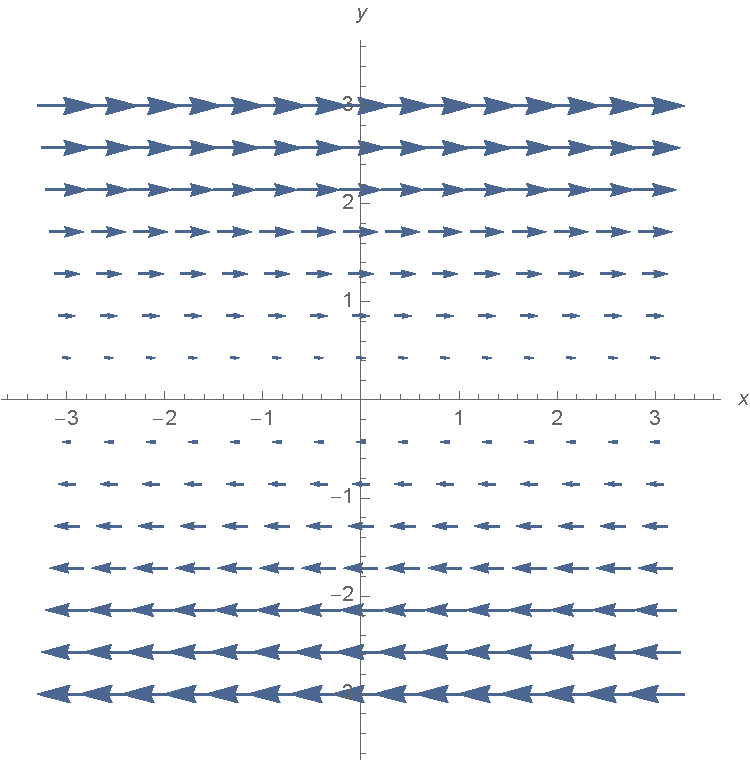
\includegraphics[width=0.45\linewidth]{figures/fig_12_4_field1.pdf}\hspace{0.1\linewidth}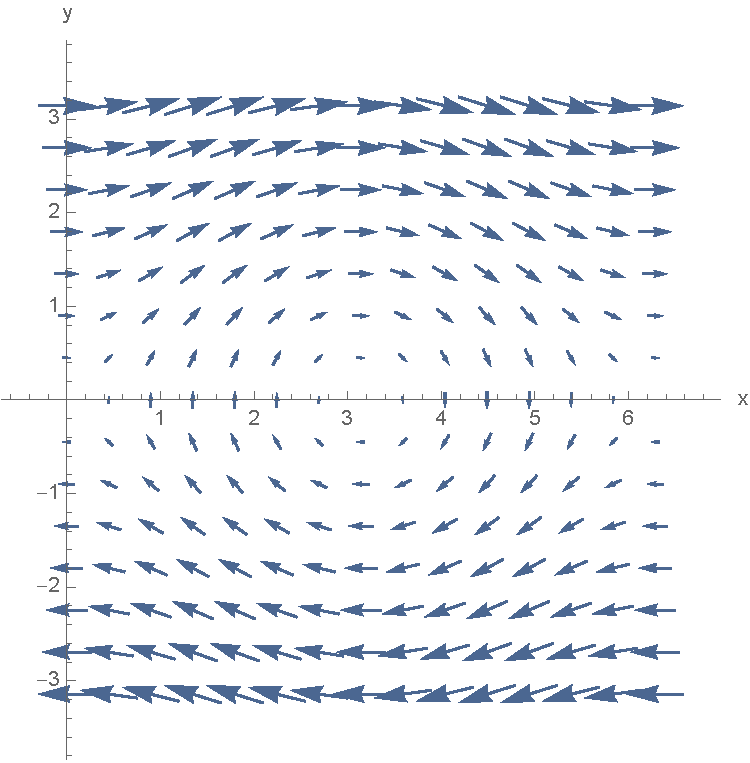
\includegraphics[width=0.45\linewidth]{figures/fig_12_4_field2.pdf}
  \caption{Two vector fields that are not path-independent.}
  \label{F:12.4.non-path-indep}
\end{figure}
\end{activity}
\begin{smallhint}

\end{smallhint}
\begin{bighint}

\end{bighint}
\begin{activitySolution}

\end{activitySolution}
\aftera
%%% Local Variables:
%%% mode: latex
%%% TeX-master: "../0_AC_MV"
%%% End:


\subsection*{What other vector fields are path-independent?}

Recall that in single variable calculus, the Second Fundamental
Theorem of Calculus tells us that given a constant $c$ and a
continuous function $f$, there is a unique function $A(x)$ for which
$A(c) = 0$ and $A'(x) = f(x)$. In particular, $A(x) = \int_c^x f(t)\,
dt$ is this function. We are about to investigate an analog of this result for
path-independent vector fields, but first we require two additional
definitions.

If $D$ is a subset of $\R^2$ or $\R^3$, we say that $D$ is
\textbf{open}\index{open!definition} provided that for every point in $D$, there
is a disc (in $\R^2$) or ball (in $\R^3$) centered at that point such
that every point of the disc/ball is contained in $D$. For example,
the set of points $(x,y)$ in $\R^2$ for which $x^2+y^2 < 1$ is open,
since we can always surround any point in this set by a tiny disc
contained in the set. However, if we change the inequality to
$x^2+y^2\leq 1$, then the set is not open, as any point on the circle
$x^2+y^2=1$ cannot be surrounded by a disc contained in the set; any
disc surrounding a point on that circle will contain points outside
the set, that is with $x^2+y^2>1$. We will also say that a region $D$
is \textbf{connected}\index{connected!definition} provided that for
every pair of points in $D$, there is a path from one to the other
contained in $D$.

\begin{activity} \label{A:12.4.5}  
  Let $\vF=\langle F_1,F_2\rangle$ be a continuous, path-independent vector field on an open,
  connected region $D$. We will assume that $D$ is in $\R^2$ and $\vF$
  is a two-dimensional vector field, but the ideas below generalize
  completely to $\R^3$. We want to define a function $f$ on $D$ by
  using the vector field $\vF$ and line integrals, much like the
  Second Fundamental Theorem of Calculus allows us to define an
  antiderivative of a continuous function using a definite
  integral. To that end, we assign $f(x_0,y_0)$ an arbitrary
  value. (Setting $f(x_0,y_0)=0$ is probably convenient, but we won't
  explicitly tie our hands. Just assume that $f(x_0,y_0)$ is defined
  to be some number.) Now for any other point $(x,y)$ in $D$, define
  \[f(x,y) = f(x_0,y_0) + \int_C\vF\cdot d\vr,\]
  where $C$ is any oriented path from $(x_0,y_0)$ to $(x,y)$. Since
  $D$ is connected, such an oriented path must exist. Since $\vF$ is
  path-independent, $f$ is well-defined. If different paths from
  $(x_0,y_0)$ to $(x,y)$ gave
  different values for the line integral, then we'd not be sure what
  $f(x,y)$ really is.

  To better understand this mysterious function $f$ we've now defined,
  let's start looking at its partial derivatives.
  \ba
\item Since $D$ is open, there is a disc (perhaps very small)
  surrounding $(x,y)$ that is contained in $D$, so fix a point $(a,b)$
  in that disc. Since $D$ is connected, there is a path $C_1$ from
  $(x_0,y_0)$ to $(a,b)$. Let $C_y$ be the line segment from $(a,b)$
  to $(a,y)$ and let $C_x$ be the line segment from $(a,y)$ to
  $(x,y)$. (See Figure~\ref{F:12.4.paths-potential}.) Rewrite $f(x,y)$
  as a sum of $f(x_0,y_0)$ and line
  integrals along $C_1$, $C_y$, and $C_x$.
  \begin{figure}
    \centering
    \begin{overpic}{figures/fig_12_4_paths_potential.pdf}
      \put(10,0){$(x_0,y_0)$}
      \put(100,117){$(a,b)$}
      \put(65,160){$(a,y)$}
      \put(160,150){$(x,y)$}
      \put(75,140){$C_y$}
      \put(125,150){$C_x$}
      \put(30,70){$C_1$}

      \put(237,0){$(x_0,y_0)$}
      \put(310,110){$(a,b)$}
      \put(387,110){$(x,b)$}
      \put(370,160){$(x,y)$}
      \put(385,140){$L_y$}
      \put(353,110){$L_x$}
      \put(257,70){$C_1$}
    \end{overpic}
    \caption{Two piecewise smooth oriented curves from $(x_0,y_0)$ to
      $(x,y)$.}\label{F:12.4.paths-potential}
  \end{figure}
\item Notice that we can parameterize $C_y$ by $\langle a,t\rangle$
  for $b\leq t\leq y$. Find a similar parameterization for $C_x$.
\item Use the parameterizations from above to write
  $\int_{C_y}\vF\cdot d\vr$ and $\int_{C_x}\vF\cdot d\vr$ as single
  variable integrals in the manner of Section~\ref{S:12.3.ParamLineIntegrals}. (Recall
  that $\vF(x,y) = \langle F_1(x,y),F_2(x,y)\rangle$, enabling you to
  express your integrals in terms of $F_1$ and $F_2$ without any dot products.)
\item Rewrite your expression for $f(x,y)$ using the single variable
  integrals above (and a line integral along $C_1$). 
\item Use your expression for $f(x,y)$ and the Second Fundamental
  Theorem of Calculus to calculate $f_x(x,y)$.
\item To calculate $f_y(x,y)$, we continue to consider a path $C_1$
  from $(x_0,y_0)$ to $(a,b)$, but now let $L_x$ be the line segment
  from $(a,b)$ to $(x,b)$ and let $L_y$ be the line segment from
  $(x,b)$ to $(y,b)$. Modify the process you used to find $f_x(x,y)$
  to find $f_y(x,y)$.
\item What can you conclude about the relationship between $\nabla f$
  and $\vF$?
\ea
\end{activity}
\begin{smallhint}

\end{smallhint}
\begin{bighint}

\end{bighint}
\begin{activitySolution}

\end{activitySolution}
\aftera
%%% Local Variables:
%%% mode: latex
%%% TeX-master: "../0_AC_MV"
%%% End:


We summarize the result of Activity~\ref{A:12.4.5} below.

\nin \framebox{\hspace*{3 pt}
  \parbox{6.25 in}{\textbf{Path-Independent Vector Fields} If $\vF$ is
  a path-independent vector field on an open, connected domain $D$,
  then $\vF$ is conservative (or a gradient vector field) on
  $D$. Furthermore, if $P$ is a point in $D$ and $f(P)$ is fixed, then
  the function \[f(Q) = f(P) + \int_C\vF\cdot d\vr\]
  (where $Q$ is a point in $D$ and $C$ is an oriented curve from $P$ to
  $Q$ in $D$) is a 
  potential function for $\vF$.} \hspace*{3 pt}} \vspace*{5pt}


%\clearpage %% Temporary just to make a handout

%\nin \framebox{\hspace*{3 pt}
%\parbox{6.25 in}{
\begin{summary}
\item Gradient vector fields are path-independent, and if $C$ is an
  oriented curve from $(x_1,y_1)$ to $(x_2,y_2)$, then $\int_C\nabla f\cdot
  d\vr = f(x_2,y_2)-f(x_1,y_1)$, with the analogous result holding if
  $f$ is a function of three variables.
\item A vector field is path-independent if and only if the
  ciruclation around every closed curve in its domain is $0$.
\item If a vector field $\vF$ is path-independent, then there exists a
  function $f$ such that $\nabla f = \vF$. That is, $\vF$ is a
  conservative or gradient vector field.
\end{summary}
%} \hspace*{3 pt}}

\nin \hrulefill

%\input{exercises/9.2.Vectors(Ex)}

\clearpage

%%% Local Variables:
%%% mode: latex
%%% TeX-master: "0_AC_MV"
%%% End:
